\documentclass[Report.tex]{subfiles}
\externaldocument[I-]{chapter_1_introduction.tex}
\externaldocument[D-]{chapter_3_discardMethod.tex}
\externaldocument[R-]{chapter_4_result.tex}
\externaldocument[C-]{chapter_5_conclusion.tex}
\externaldocument[RE-]{chapter_6_recognition.tex}

\begin{document}
\chapter{Method}
\label{chap:Method}
\section{Description}
The following section as mentioned in Section~\ref{subsec:Report Layout} will present our methods. Bellow we present each component individually and the corresponding methods for them. A short description on what challenges have to
be solved for each component will be addressed first.

\section{Component: Text segmentation}
\label{Method:Text_segmentation}

\subsection{Description}
In this part of the program, we want to be able to segment out text segments in the image. Afterwards we want to segment out lines and letter for further classification, see section \nameref{subsec:Find_line} and \nameref{subsec:Find_Symb} for reference. In this part we assume that the images have black text on white background, and they mostly consists of text.

\begin{flushleft}
  \subsubsection{Approach: Simple Image Analysis Technics}
  Our approach here was inspired by this online blog \href{https://www.danvk.org/2015/01/07/finding-blocks-of-text-in-an-image-using-python-opencv-and-numpy.html}{Source}\cite{_finding_????}. We simplified the original approach to the following steps:
  \begin{enumerate}
    \item \textbf{Find Edges/Outliners of the image.}
    Initial idea is to use Canny, but we found Morphological Gradient to perform better. It indicates the contrast of the edges, so we can get better differences in some natural images (as long as the text and background are close to black and white respectively).
    \item \textbf{Otsu Thresholding.}
    We need our image to be a binary image. We simply use OpenCV Otsu algorithm to achieve it that.
    \item \textbf{Morphological Closing.}
    Since we want line segments we use Morphological Closing with large horizontal filter to merge as many horizontal letters together as possible.
    \item \textbf{Extract Regions}
    OpenCv FindContours was used to find the different text regions. We then exclude regions which are smaller than a selected threshold. The different region are return as coordinate of the different rectangular boxes.
  \end{enumerate}
\end{flushleft}

\section{Component: Preprocessing}
\label{Method:Preprocessing}
\subsection{Description}
Definition of preprocessing; the act of preparing the data for further use,
in our case for classification. \par
After the text segmentation we assume we have an image consisting of white text on black background. What remains for us to do is to segment out each character and format it to the right data type for the classifier. Hence the challenges we will have to solve here are:


\begin{flushleft}
  \textbf{Challenges}
  \begin{itemize}
    \item{Data formatting/casting}
    \begin{itemize}
      \item{The data we want to test a classifier on needs to match the data we trained our classifier with. Hence we need to format our data to the same format as the datasets. No need for a specific approach.}
    \end{itemize}
    \item{Rotated text}
    \begin{itemize}
      \item{Our approach for character segmentation needs text rotated horizontally.}
    \end{itemize}
      \item{Line segmentation}
    \begin{itemize}
      \item{Our approach for character segmentation needs lines as input, as a sequence of lines on top of each other breaks the algorithm.}
    \end{itemize}
      \item{Character segmentation}
    \begin{itemize}
      \item{We need to segment each character because the classifier cannot distinguish several characters from one image.}
    \end{itemize}
  \end{itemize}
\end{flushleft}

\subsection{Find rotation}
\begin{flushleft}
  \textbf{Approach: OpenCV minAreaRect() + CNN solution} \\
  This approach uses \href{https://en.wikipedia.org/wiki/Convex_hull}{convex hull}
  to find the convex hull of the text, and then
  \href{https://en.wikipedia.org/wiki/Rotating_calipers}{rotating calipers} to
  find the minimum area rectangle. \par
  One important note here is that the method above operates on binary images, therefor we need to convert our image to binary, possibly using some threshold algorithm. \par
  cv.minAreaRect returns text rotated in one of following angles [0\textdegree, 90\textdegree, 180\textdegree, 270\textdegree], see Figure~\ref{fig:4angle_rot} for illustration. We will use a CNN to determine which of the angles is correct and then rotate it accordingly.
  To train the network we needed a dataset with the corresponding angles as labels, as we couldnt find one, we decided to create it ourself. We describe our approach later in this document.

  \begin{enumerate}
    \item \textbf{Binary image}
    For the Convex hull algorithm to work, the text segment and the background needs to be distinguishable. Convert image to a binary image using OpenCV threshold function and/or bitwise\textunderscore not to flip foreground and background colors.
    \item \textbf{cv.minAreaRect()}
    Feed our newly generated image to cv.minAreaRect.
    \item \textbf{CNN solution - find correct rotation}
    Now that we have text rotated in one of [0\textdegree, 90\textdegree, 180\textdegree, 270\textdegree], we have several options finding the correct angle of the text segment.
    \begin{enumerate}
	\item{The most straightforward approache would be to find the rotation of first character and rotate the whole segment accordingly (fast and naive)}
	\item{Pick N characters and find their rotation, angle with most matches will be our final angle of rotation. This is somewhat slower (depends on N) but gives us bit more confidence than (a)}
	\item{Finally we can classify the angle of each individual character before we try to determine the correct angle based on the results. This gives us the highest accuracy but on the cost of time/computation power. This is the only approach able to successfully recognize this type of text: (find better example)\LaTeX}
	\end{enumerate}
    \end{enumerate}
\end{flushleft}


\subsection{Find line}\label{subsec:Find_line}
After all the preprocessing done up til this point we have rotated segment of text. At this point it is enough to just use projection histogram. We basically sum number of active pixels in each row and end up with one dimensional array with same size as image height, one value for each row in input image.
E.g. [0 0 0 0 0 5 12 18 20 15 11 0 0 0 0 5 7 8..], this will mean there are some data (most likely text) between 5th and 10th row, and 15th  up to another line break. EXAMPLES SHOULD FOLLOW

\subsection{Find Symbol/Letter Segmentation}\label{subsec:Find_Symb}
Letter segmentation was similar to Text Segmentation. We added a few steps and removed the morphology part. The additional step was to fill holes in the image, example like 8 and O can give multiple wrong contour. cv2.floodFill was used to solve this problem.
\begin{enumerate}
  \item Do threshold.
  \item Inverse the image since we work on black text on white background.
  \item Do morphological dilation with long vertical kernel, This is to include the dot in 'i'.
  \item Add a bolder around the line-image, that is separate elements from edge after previous step. This is to make cv2.floodFills work.
  \item Fill any holes, cv2.floodFills.
  \item Use FindContours
  \item Ignore element where contour size smaller than a threshold(half the letter size), to ignore ',','.' and other non letter element.
\end{enumerate}


\section{Component: Classification}
\label{Method:Classification}
\begin{flushleft}
  \textbf{Description} \\
  For the classification component there where only 2 approaches we considered,
  Convolutional Neural Network (CNN), the architecture is illustration in
  Figure~\ref{fig:CNN_architecture}, and a Multilayer Perceptron (MLP or Deep
  neural network (DNN)), Figure~\ref{fig:neural_net2}. However the method we ended up choosing for the final result is CNN. In
  Section~\nameref{Method:Classification} we explain why we discarded
  the MLP approach. \par
\end{flushleft}

\begin{flushleft}
  \textbf{Convolutional Neural Network} \\
  The basic idea of a CNN is train some number of filters and then
  after the filters are trained, run the image which is now ``filterd'', through
  a fully connected network. The fully connected network will then try and
  classify based on the feature images from the filtering/convolution layers. \par
  A short description of key points of a CNN, the architecture and variable choices we have made for the CNN, is presented below
\end{flushleft}

\begin{figure}[H]
  \centering
  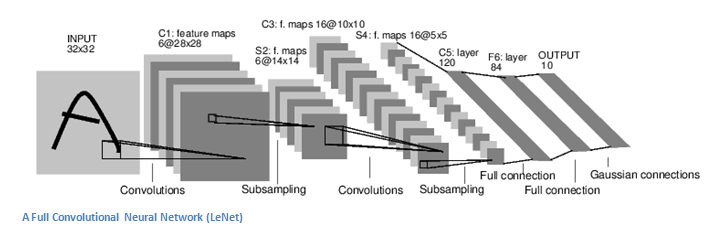
\includegraphics[height=4cm]{res/LeNet.png}
  \caption{Convolutional Neural network \href{https://adeshpande3.github.io/A-Beginner\%27s-Guide-To-Understanding-Convolutional-Neural-Networks/}{Source}}
  \label{fig:CNN_architecture}
\end{figure}

\begin{flushleft}
  \textbf{CNN - Basics} \\
  \begin{itemize}
   \item{Convolutional layer}
   \begin{itemize}
    \item{This layer consists of several filters/kernels that are convolved over the image and based on how many filters one uses, the same amount of feature images are made. The purpose of the filters are to grasp some spatial characteristics of the image, and make it available for further processing.
    The filters here correspond to the weights in the MLP, these are first initialized at random (or with a smart initialization method), then these will be updated as the network is trained.
First layer filters are able to spot simple geometry like straight or curved lines, but the deeper we dive into networks topology the more complex shapes the filters can recognize. It is not unusual that last layers on large networks can differenciate between faces, animals, objects.\par
    In a CNN we can have arbitrary many convolutional layer and arbitrary many filters at each layer. However just like a regular MLP, increasing the number of layers and or filters; can allow the network to fit the training data arbitrarily well, unfortunately at the cost of processing time, mostly during training, but also during prediction phase.}
   \end{itemize}
   \item{Pooling}
   \begin{itemize}
    \item{The pooling layer allows us to downsize the data. This makes it possible to start with images which are relatively big, and as it's data propagates through the network we downsize it. As for the convolution layer the pooling layer can be used arbitrarily many times in a network.
    Pooling makes our network rotation invariant to minor changes in angle, as outputs max/min value of a (pooling-size) block regardless of where in the block this value is.}
   \end{itemize}
   \item{Fully connected layers (FC)}
   \begin{itemize}
    \item{This layer works basically the same way as the hidden layers in an MLP.
    The output of last convolution layer is then flattened and send to N fully connected layers (also sometimes referenced as dense layer). At the last layer we have same number of outputs as we have classes, just like in regular MLP.}
   \end{itemize}
  \end{itemize}
\end{flushleft}

\todo[inline]{Architecture description should follow, choices of variables too \\
. \\
. \\
. \\
. \\
}


\section{Component: Datasets}
\label{Method:Datasets}

\todo[inline]{include only datasets we have used for the final software \\
Remove MNIST from this place, and moove it to chapter 3 discardMethod}

\subsection{Description}

\begin{flushleft}
  In order to learn our network to distinguish between the characters it needs training. Training is done by feeding images of known objects to the network (labeled data) and telling it how inaccurate it's prediction so that network can adjust it's weights accordingly. This type of training is called supervised training as we guide our network during training process.
For network to get high accuracy of prediction a lot of labeled data is needed. Lucky for us datasets like MNIST exists, more info about it later.
\end{flushleft}

\begin{flushleft}
  \textbf{Limitation - proof-of-concept} \\
  As we have limited us to the digits and English alphabet, we will need labeled data for each of these [0..9] + 36 characters; divided into training, test and validation sets. As the concept of classifying only numbers vs all 36 characters does not differ that much, we will first see if we can solve the OCR problem with just numbers. Therefore we only need a dataset containing numbers at first. After that we can proceed our search for a dataset containing all the characters we need.
\end{flushleft}

\begin{flushleft}
  \textbf{Dataset} \\
  \textbf{MNIST} \\
  This is a dataset containing images of handwritten digits [0-9]. It has a training set of 60.000 examples and a test set of 10.000 examples. Training set is further divided into 55000 examples of actual training set, while 5000 images are treated as validation set (this number can be changed depending which interface we use to access MNIST data).
MNIST dataset is compressed into 4 binary *.gz files, but we dont need to implement any readers/parsers ourself as tensorflow already has two we can choose between.
(ref. reader to http://yann.lecun.com/exdb/mnist/).
\end{flushleft}
\end{document}
